\documentclass{book}
\usepackage[english]{babel}
\usepackage{graphicx}
\usepackage{hyperref}
\begin{document}

\title{\TeX4ht\ Template for Online Books}
\author{Michal Hoftich}
\maketitle
\tableofcontents

\chapter{Introduction}



\chapter{Basic Usage}

\section{Create a New Github Repository}
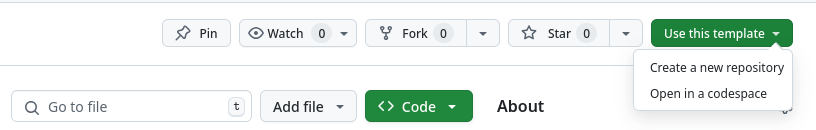
\includegraphics[width=\textwidth]{img/template-use.png}

To start your own online book using this template, click the "Use this
template" button at the top of the GitHub repository page. This will create a
new repository in your account with the same structure and files. You can then
clone it, customize the content, and start building your own slides and
handouts.






\chapter{Compiling the Book}


You can compile the output files using any standard \LaTeX\ distribution which includes \href{https://www.tug.org/tex4ht/}{\TeX4ht}.

\begin{verbatim}
$ make4ht -l book.tex    
\end{verbatim}

The \verb|-l| option  ensures that Lua\LaTeX\ is used as the compiler. 


The HTML version is built from the article-style handout, not the Beamer slides.
This makes it better suited for the web or long-term sharing, since it includes
all explanations and doesn’t depend on slide layout.

\chapter{Automated HTML Output}

This chapter explains how \href{https://docs.github.com/en/actions/writing-workflows/quickstart}{GitHub Actions}
is used to automatically generate and publish an HTML version of the handout whenever changes are pushed to the \texttt{main} branch.

The output is built using \texttt{make4ht} and published to the \texttt{gh-pages} branch,
making it easy to share a web-readable version of the talk.

Key parts of the workflow that builds and publishes the HTML:

\begin{verbatim}
- name: Run make4ht
  uses: xu-cheng/texlive-action/full@v1
  with:
    run: |
      make4ht -lj index -a debug -d out book.tex

- name: Publish the web pages
  uses: peaceiris/actions-gh-pages@v3
  with:
    github_token: ${{ secrets.GITHUB_TOKEN }}
    publish_dir: ./out
\end{verbatim}



The workflow is defined in the \texttt{.github/workflows/main.yml} file.
You can edit this file to customize the build process, such as changing the options passed to \texttt{make4ht}.

It uses two GitHub Actions: \href{https://github.com/xu-cheng/texlive-action}{xu-cheng/texlive-action}
and \href{https://github.com/peaceiris/actions-gh-pages}{peaceiris/actions-gh-pages}.
The first one lets you use any command available in the TeX Live installation, such as \texttt{make4ht} or \texttt{lualatex}.
The second one publishes the contents of a specified directory to the \texttt{gh-pages} branch of your repository,
which is used by GitHub Pages to serve static content.



\section{Automatic HTML Build}
Changes pushed to \texttt{main} branch trigger a GitHub Actions workflow that:

\begin{itemize}
  \item Compiles \texttt{handout.tex} to HTML using \texttt{make4ht}
  \item Publishes the output to the \texttt{gh-pages} branch
\end{itemize}

The following command is used for the compilation:

\begin{verbatim}
make4ht -lj index -a debug -d out handout.tex
\end{verbatim}


This builds the HTML into the \texttt{out/} folder, which is then published
using the \texttt{peaceiris/actions-gh-pages} action, specified by the
\texttt{publish\_dir} setting.


\paragraph{Why \texttt{-j index}?}
\begin{itemize}
  \item The \texttt{-lj index} option is a shorthand for \texttt{-l -j index}
  \item The \texttt{-j index} option sets the HTML output filename to \texttt{index.html}
  \item This lets you use clean URLs like:
  
\begin{verbatim}
https://username.github.io/repo/
\end{verbatim}

\end{itemize}


There’s no need to specify the filename in the link — GitHub Pages
automatically looks for \texttt{index.html} by default. This makes it easier to share
the presentation and helps avoid broken links due to filename mismatches.

For example, this book is available at: \url{https://michal-h21.github.io/tex4ht-booksite/}.

\chapter{Github Pages}

\section{Github Actions Interface}
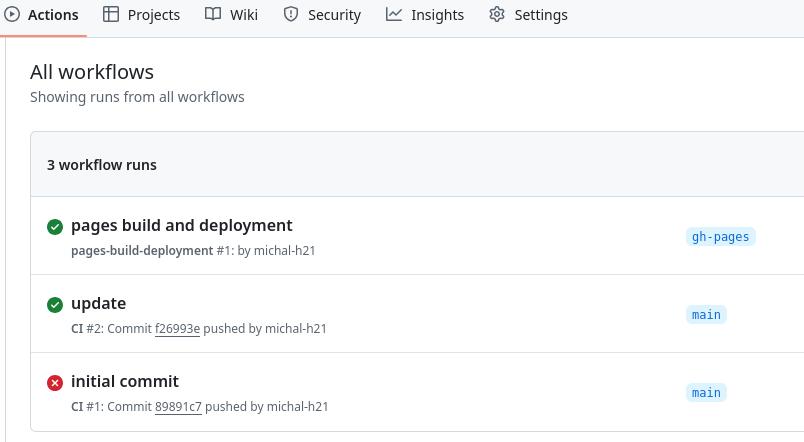
\includegraphics[width=\textwidth]{img/github-actions.png}

After you push changes to the \texttt{main} branch, you can check the \texttt{Actions} tab in your
Github repository. It shows the status of the workflow, including whether it ran successfully or if there were any errors.


\section{Errors}
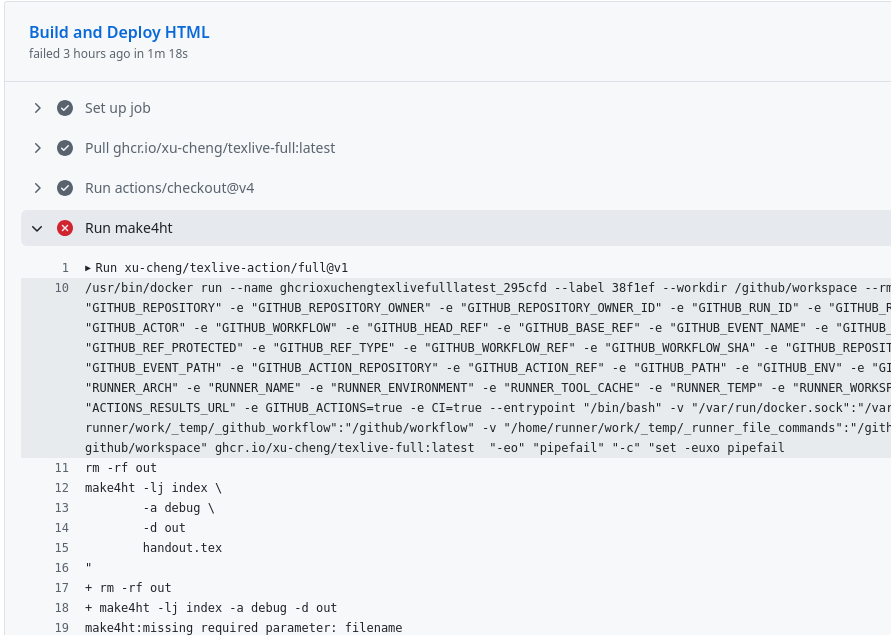
\includegraphics[width=\textwidth]{img/github-error.png}


You can also check the logs of the workflow run to see what went wrong.
If you encounter an error, it will be displayed in the logs, and you can use that
information to debug the issue.

In this case, the filename of the TeX file was incorrect. I had to fix the filename in the GitHub Actions YAML file.


\section{Setup Github Pages}
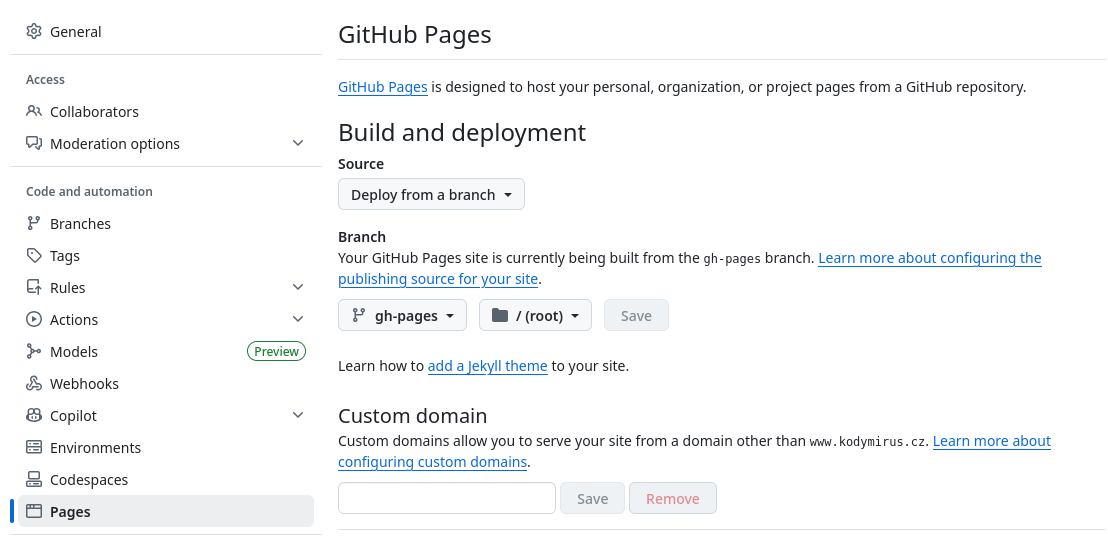
\includegraphics[width=\textwidth]{img/github-pages.png}

Once the workflow runs successfully, you can set up GitHub Pages to serve the \texttt{gh-pages} branch.

All output files produced by \texttt{make4ht} will be served on the web.
They will be available at:
\verb|https://username.github.io/repo/|,
where \texttt{username} is your GitHub username and \texttt{repo} is the name of your repository.
\end{document}
